% -*- root: ../../main.tex -*-
\section{Client Server}
\label{sec:client_server_design}
La realizzazione della modalità di gioco \textbf{multiplayer} richiede di elaborare una struttura che permetta a due o più giocatori di interagire \textbf{contemporaneamente} con la medesima partita.

Come introdotto in \ref{subsec:client_server} si è scelto di realizzare un sistema multi-giocatore con le seguenti caratteristiche:
\begin{itemize}
    \item I giocatori interagiscono con il gioco da \textbf{istanze separate}.
    \item La gestione del sistema è \textbf{centralizzata} e la partita è gestita da un \textbf{Server}.
\end{itemize}

\begin{figure}[H]
	\centering
	\includegraphics[width=0.99\columnwidth]{drawio/client-server/Controller-Actors-Interaction.pdf}
	\caption{Diagramma delle classi che rappresenta le connessioni tra il Controller e gli attori Client e Server.}
	\label{fig:Controller-Actors-Interaction}
\end{figure}

Per gestire l'\textbf{interazione} tra il Server e i Client era necessario disporre di un \textbf{canale di comunicazione} tra di essi. Per concretizzare ciò si è scelto di utilizzare un approccio ad \textbf{attori}, introducendo \texttt{ClientActor} e \texttt{ServerActor}.
La \textbf{modellazione} dell'architettura \textbf{Client-Server} è stata realizzata come raffigurato in \ref{fig:Controller-Actors-Interaction}.

La struttura del diagramma si presenta con due elementi principali: gli \textbf{attori} e il \textbf{Controller}.
\begin{itemize}
    \item \textbf{Controller:} rappresenta il punto di \textbf{snodo} dello schema ed espone, tra le altre cose, i metodi necessari per gestire le informazioni che arrivano dal \texttt{ClientActor} o dal \texttt{ServerActor}, a seconda della modalità in cui si vuole giocare.
    \item \textbf{Attori:} \texttt{ClientActor} e \texttt{ServerActor} sono intesi come \textbf{interfaccia di comunicazione} tra il sistema presente nell'istanza di gioco che agisce come \textbf{Server} e quello presente nelle istanze in funzione sui \textbf{Client}. I due attori comunicano mediante \textbf{scambio di messaggi}.
\end{itemize}

\subsection{Assetto Client-Server} 
Il diagramma delle classi è stato progettato promuovendo un'idea di \textbf{flessibi-lità}. A seconda della modalità di gioco scelta, l'assetto deve poter \textbf{variare} per permettere una gestione \textbf{efficiente} delle dinamiche del sistema.
    \subsubsection{Modalità Client}
        Nella modalità Client la struttura delle classi è la seguente:
        \begin{itemize}
            \item L'\texttt{Engine} del gioco \textbf{non viene utilizzato} e pertanto risulta slegato dal Controller.
            \item Il Controller \textbf{crea} e \textbf{mantiene} un'istanza del \texttt{ClientActor}.
            \item Il \texttt{ServerActor} è \textbf{assente}.
        \end{itemize}

    \subsubsection{Modalità Server}
    Quando il sistema passa in modalità Server, viene assunto un assetto diverso che si presenta in questo modo:
        \begin{itemize}
            \item Il Controller \textbf{crea} e \textbf{mantiene} un'istanza del \texttt{ServerActor}.
            \item Il \texttt{ClientActor} è \textbf{assente}.
            \item L'\texttt{Engine} del gioco viene \textbf{mantenuto}, poiché dovrà occuparsi completamente della gestione della partita in corso.
        \end{itemize}    
        
\subsection{Gestione della comunicazione}
Ottenuta la configurazione relativa al \textbf{ruolo} scelto è possibile gestire i \textbf{flussi} di comunicazione che vanno dal \textbf{Client} al \textbf{Server} e viceversa.
    \paragraph{Gestione in entrata:}
    ciascun \textbf{attore}, nel momento in cui \textbf{riceve} un messaggio dalla sua controparte esterna, chiama, sul \textbf{Controller}, il \textbf{metodo} preposto alla gestione dello stesso.
    
    Ad esempio, alla ricezione di un messaggio che indica l'inizio del gioco, il \texttt{ClientActor} dovrà chiamare il metodo \texttt{notifyGameStart()} sull'istanza di \texttt{ActorController} da esso \textbf{mantenuta internamente}.
    
    \paragraph{Gestione in uscita:}
    nel momento in cui, invece, è il sistema locale a dover \textbf{aggiornare} la controparte esterna su qualcosa, il flusso si inverte: il \textbf{Controller}, a fronte di un \textbf{evento}, chiama sull'attore il \textbf{metodo} preposto alla gestione dello stesso. 
    
    Ad esempio, alla pressione di un tasto da parte dell'utente, il Controller chiamerà il metodo \texttt{handle()} esposto dalla sua istanza di \texttt{ClientActor}, passando come parametro un \texttt{CommandEvent}. All'interno di questo metodo verrà eseguita una \texttt{send} che permetterà di inviare un messaggio al Server esterno al fine di notificare la ricezione del comando. 


\subsection{Sequenze di interazioni}
La gestione dell'\textbf{inizio}, dello \textbf{svolgimento} e dell'\textbf{arresto} di una partita \textbf{multiplayer} si svolge attraverso una serie di \textbf{fasi} di interazione tra gli elementi in gioco. Queste interazioni sono state evidenziate nel diagramma in \ref{fig:sequenceClientServer}

Le fasi di interazione possono essere raggruppate in tre \textbf{macro-fasi}:
\begin{enumerate}
    \item \textbf{Setup:} prima di cominciare una partita è necessaria una prima fase di \textbf{configurazione} che si svolge nel seguente modo:
        \begin{enumerate}
            \item Inizialmente si ha che un'istanza del gioco assume il ruolo di \textbf{Server}, mentre una o più altre istanze scelgono il ruolo di \textbf{Client}
            \item Prima di iniziare il gioco, il giocatore che si trova sull'istanza Server sceglie il \textbf{numero di giocatori} e configura le \textbf{impostazioni della partita}.
            \item Il Server rimane in \textbf{attesa delle richieste di join} provenienti dai Client.
            \item Ad ogni richiesta di \texttt{join} ricevuta, il Server \textbf{controlla} se è stato raggiunto il \textbf{numero massimo di giocatori}. In caso affermativo \textbf{respinge} la richiesta, altrimenti la \textbf{accoglie}.
            \item Quando vi è un \textbf{numero corretto} di Client collegati e quando questi si trovano tutti nello stato \texttt{ready}, il Server può \textbf{avviare} la partita.
        \end{enumerate}
    \item \textbf{Gioco:} è la fase principale dove avvengono interamente le dinamiche di gioco e consiste nella ripetizione ciclica di tre step.
        \begin{enumerate}
            \item Ciascun Client invia al Server la propria azione, derivante dal \textbf{comando} impartito dal proprio utente.
            \item Il Server \textbf{riceve} i comandi e li \textbf{elabora} insieme ai propri.
            \item Il Server calcola il \textbf{nuovo mondo} e lo invia a tutti i Client.
        \end{enumerate}
    \item \textbf{Arresto:} quando la partita giunge al termine avvengono le seguenti interazioni:
        \begin{enumerate}
            \item Il Server calcola i \textbf{punteggi}
            \item Il Server \textbf{invia l'esito} della partita a tutti Client.
            \item Le \textbf{connessioni} tra il Server e i Client vengono \textbf{chiuse}
        \end{enumerate}
\end{enumerate}

\begin{figure}[H]
	\centering
	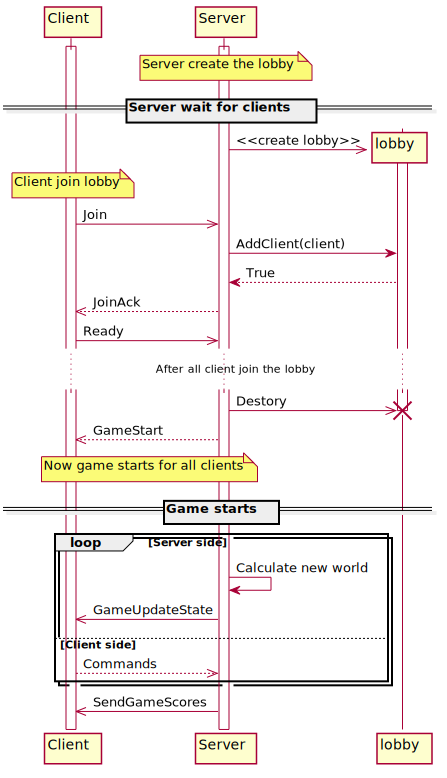
\includegraphics[width=0.80\columnwidth,height=0.95\linewidth]{plantuml/rendered/sequenceDiagrams/sequenceClientServer.pdf}
	\caption{Diagramma di sequenza che rappresenta la fase di join alla partita e lo svolgimento di essa.}
	\label{fig:sequenceClientServer}
\end{figure}







